\section{相关平均的误差区间}
\label{sec:mcerr-chain-interval}

独立样本的渐近误差区间由三块拼成：中心极限定理给出正态极限，样本方差一致地估计极限方差，Slutsky定理把两者合在一起。链平均要得到类似的区间，三块都要重新检查。正态极限不再由独立性自动保证；极限方差变成了长期方差$\sigma_{\mathrm{LR}}^{2}$，样本方差不再适用；此外，链是否已经到过目标的重要区域，单凭记录无法确认。本节依次处理这三点。

\subsection{链平均的正态近似}
\label{sec:mcerr-chain-clt}

先在有限状态空间上看清楚正态极限需要什么条件。设链的状态集$\mathcal{X}$有限，转移概率为$K(x,y)$。若对任意两个状态$x,y$，从$x$出发都能以正概率在有限步内到达$y$，称链\term{不可约}（irreducible）；若对每个状态$x$，所有满足$K^{t}(x,x)>0$的步数$t$的最大公因子为$1$，称链\term{非周期}（aperiodic）。不可约保证链不会被困在一部分状态里，非周期保证它不会在几组状态之间按固定节拍轮转。

卷九将证明：有限、不可约且非周期的链有唯一的不变分布$\pi$，并且从任意初值出发，$K^{t}(x,\cdot)$以几何速度趋于$\pi$：存在$C<\infty$与$r<1$，使$d_{\mathrm{TV}}(K^{t}(x,\cdot),\pi)\leq Cr^{t}$对所有$x$成立。由此可得$\lvert\gamma_k\rvert\leq C'r^{k}$，长期方差的级数绝对收敛。在这个基础上有下面的定理。

\begin{theorem}[有限状态链的中心极限定理]
\label{thm:mcerr-finite-clt}
设链的状态集有限，不可约且非周期，不变分布为$\pi$。则对任意$f\colon\mathcal{X}\to\mathbb{R}$与任意初始分布，
\begin{equation}
 \sqrt{N}\,\bigl(\hat{I}_N-I\bigr)\xrightarrow{\mathrm{d}}\mathcal{N}\bigl(0,\sigma_{\mathrm{LR}}^{2}\bigr) ,
 \label{eq:mcerr-finite-clt}
\end{equation}
其中$\sigma_{\mathrm{LR}}^{2}$由式~\eqref{eq:mcerr-long-run}按平稳链计算；$\sigma_{\mathrm{LR}}^{2}=0$时极限理解为$0$处的单点分布。
\end{theorem}

这个定理的证明需要卷九才系统建立的鞅工具，这里说明它的机制。对有限不可约链，方程$g(x)-\sum_yK(x,y)g(y)=f(x)-I$总有解$g$。记$Kg(x)=\sum_yK(x,y)g(y)$，把$f-I=g-Kg$代入部分和并错开一项，
\[
 \sum_{t=1}^{N}\bigl(f(X^{(t)})-I\bigr)=\sum_{t=1}^{N}D_t+Kg(X^{(0)})-Kg(X^{(N)}),\qquad D_t=g(X^{(t)})-Kg(X^{(t-1)}) .
\]
有限状态上$g$有界，末尾两项除以$\sqrt{N}$后趋于零。每个$D_t$在给定此前全部状态时条件均值为零：链在这些增量上不再“记得”过去的方向。这样的增量和满足与独立和类似的中心极限定理，增量的平稳方差恰好等于$\sigma_{\mathrm{LR}}^{2}$。完整的论证可参考\BookChapterRef{chap:discrete-time-stochastic-processes}{卷九第3章“离散时间随机过程”}。

\paragraph{两状态链}
取状态$\{0,1\}$，$K(0,1)=a$，$K(1,0)=b$，$0<a+b<2$，$f$为状态$1$的示性函数，如图~\ref{fig:mcerr-two-state}(a)。记$p_k=\mathbb{P}(X^{(k)}=1)$，一步转移给出
\[
 p_{k+1}=(1-b)\,p_k+a\,(1-p_k)=a+\lambda p_k,\qquad \lambda=1-a-b .
\]
不动点是$\pi_1=a/(a+b)$，且$p_{k+1}-\pi_1=\lambda(p_k-\pi_1)$。从状态$1$出发，$p_0-\pi_1=\pi_0$，所以
\[
 \mathbb{P}\bigl(X^{(k)}=1\mid X^{(0)}=1\bigr)=\pi_1+\pi_0\lambda^{k} .
\]

平稳时，自协方差为
\[
 \gamma_k=\pi_1\bigl(\pi_1+\pi_0\lambda^{k}\bigr)-\pi_1^{2}=\pi_0\pi_1\lambda^{k} ,
\]
求和得到
\begin{equation}
 \sigma_{\mathrm{LR}}^{2}=\pi_0\pi_1\Bigl(1+\frac{2\lambda}{1-\lambda}\Bigr)=\pi_0\pi_1\,\frac{1+\lambda}{1-\lambda} .
 \label{eq:mcerr-two-state-lrv}
\end{equation}
取$a=0.1$，$b=0.2$：$\pi=(2/3,1/3)$，$\lambda=0.7$，$\gamma_0=2/9\approx0.222$，
\[
 \sigma_{\mathrm{LR}}^{2}=\frac29\times\frac{1.7}{0.3}=\frac{34}{27}\approx1.259,\qquad \frac{N_{\mathrm{eff}}}{N}=\frac{0.3}{1.7}\approx0.176 .
\]
图~\ref{fig:mcerr-chain-clt}(a)从状态$0$出发运行$20000$条长度$N=2000$的链，$\sqrt{N}(\hat{I}_N-1/3)$的样本方差为$1.267$，直方图贴合$\mathcal{N}(0,34/27)$。若误用单个函数值的方差$2/9$，区间会窄到应有宽度的$\sqrt{(2/9)/(34/27)}\approx0.42$倍。

\begin{BookInlineFigure}
 \centering
 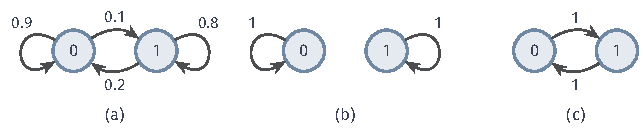
\includegraphics[width=109mm]{figures/07-probability/08-sampling-and-integration/tikz/mcerr-two-state/figure.pdf}
 \caption{两状态链的转移图，箭头上的数为转移概率。(a)$a=0.1$，$b=0.2$，不可约且非周期；(b)$a=b=0$，两个状态各自吸收，链可约；(c)$a=b=1$，不可约但周期为$2$。}
 \label{fig:mcerr-two-state}
\end{BookInlineFigure}

图~\ref{fig:mcerr-two-state}(b)与(c)是条件不成立的两种情形。可约链（$a=b=0$）就是上一节始终停在原地的例子，$\hat{I}_N=f(X^{(0)})$，既不趋于$I$，也没有正态极限。周期链（$a=b=1$）在$0,1$之间严格交替，从$\pi$出发时$\lambda=-1$，式~\eqref{eq:mcerr-two-state-lrv}给出$\sigma_{\mathrm{LR}}^{2}=0$：$N$为偶数时$\hat{I}_N$恰好等于$1/2$，误差比$N^{-1/2}$小得多，正态近似退化。从固定的状态$0$出发时，$X^{(t)}$的分布在两个单点之间来回切换，永远不趋于$\pi$，时间平均却仍然收敛。可见非周期性主要关系到边缘分布的收敛，不可约性关系到时间平均能否看到整个目标。

\paragraph{一般状态空间}
状态连续时，“以几何速度趋于目标”需要允许依赖初值的常数。若存在$r<1$与函数$M(x)$，对$\pi$几乎所有的$x$有$M(x)<\infty$，且
\begin{equation}
 d_{\mathrm{TV}}\bigl(K^{t}(x,\cdot),\pi\bigr)\leq M(x)\,r^{t},\qquad t=1,2,\dots ,
 \label{eq:mcerr-geometric-ergodic}
\end{equation}
就称链\term{几何遍历}（geometrically ergodic）。式中$t$步后的转移分布与目标之间的总变差按几何速度衰减，衰减的比例不依赖初值，起点越远只是常数$M(x)$越大。

链~\eqref{eq:mcerr-ar1}是几何遍历的。由式~\eqref{eq:mcerr-ar1-marginal}，$K^{t}(x,\cdot)$与$\pi$只差均值$\rho^{t}x$和方差$1-\rho^{2t}$。图~\ref{fig:mcerr-geo-ergodic}用数值积分算出$\rho=0.9$时的总变差：从$x=3$与$x=10$出发，曲线最终与$0.9^{t}$平行，起点越远曲线越高；从$x=0$出发，均值没有偏离，只剩方差的差别，衰减得更快，按$0.81^{t}$下降。

\begin{BookInlineFigure}
 \centering
 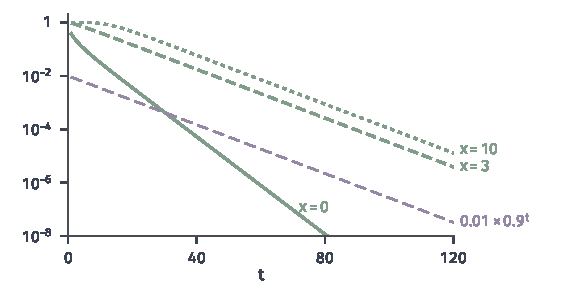
\includegraphics[width=96mm]{figures/07-probability/08-sampling-and-integration/matplotlib/mcerr-geo-ergodic/figure.pdf}
 \caption{链~\eqref{eq:mcerr-ar1}在$\rho=0.9$时，$t$步转移分布$\mathcal{N}(0.9^{t}x,1-0.81^{t})$与$\mathcal{N}(0,1)$的总变差（数值积分），绿色实线、虚线、点线分别为$x=0,3,10$；紫色虚线为参考斜率$0.01\times0.9^{t}$，纵轴为对数刻度。}
 \label{fig:mcerr-geo-ergodic}
\end{BookInlineFigure}

几何遍历配合比二阶稍强的矩条件，就足以给出正态极限。

\begin{theorem}[几何遍历链的中心极限定理]
\label{thm:mcerr-geo-clt}
设链以$\pi$为不变分布且几何遍历，$f$满足$\mathbb{E}_{\pi}\lvert f\rvert^{2+\delta}<\infty$，其中$\delta>0$。则平稳自协方差绝对可和，$\sigma_{\mathrm{LR}}^{2}<\infty$，并且链从$\pi$出发时
\begin{equation}
 \sqrt{N}\,\bigl(\hat{I}_N-I\bigr)\xrightarrow{\mathrm{d}}\mathcal{N}\bigl(0,\sigma_{\mathrm{LR}}^{2}\bigr) .
 \label{eq:mcerr-geo-clt}
\end{equation}
\end{theorem}

证明要估计相隔$k$步的两个函数值之间的依赖如何随$k$衰减，再用前面提到的鞅增量分解，篇幅较长，读者可查阅~\scite{math-meyn2009markov}。在卷九所讨论的常返条件下，结论对任意初始分布也成立。矩条件中的$\delta$一般不能取为零：对某些几何遍历的链，只满足$\mathbb{E}_{\pi}[f^{2}]<\infty$的$f$可以使$\sigma_{\mathrm{LR}}^{2}=\infty$，这类反例的构造较复杂。对链~\eqref{eq:mcerr-ar1}，$f(x)=x$或$x^{2}$的各阶矩都有限，定理适用，$f(x)=x$的极限方差就是$19$。

\paragraph{可和协方差不足以给出正态极限}
第~\ref{sec:mcerr-long-run}小节的方差极限只用了协方差绝对可和。下面的例子说明，仅有这一条不能推出正态极限。链的状态是一对$(W,Y)$。初始时$W$以各$1/2$的概率取$1$或$3$，此后永不改变；每一步$Y$重新抽取为$W\varepsilon$，其中$\varepsilon\sim\mathcal{N}(0,1)$与过去独立。转移核是
\[
 K\bigl((w,y),\cdot\bigr)=\delta_{w}\otimes\mathcal{N}(0,w^{2}) ,
\]
不变分布是“$W$各以$1/2$取$1,3$，给定$W$后$Y\sim\mathcal{N}(0,W^{2})$”。

取$f(w,y)=y$，$I=0$。平稳时
\[
 \gamma_0=\mathbb{E}[W^{2}]=5,\qquad \gamma_k=\mathbb{E}\bigl[W^{2}\varepsilon_0\varepsilon_k\bigr]=0\quad(k\geq1) ,
\]
自协方差除$\gamma_0$外全为零，绝对可和，长期方差$\sigma_{\mathrm{LR}}^{2}=5$，而且$N\operatorname{Var}(\hat{I}_N)$对每个$N$都等于$5$。可是
\[
 \sqrt{N}\,\hat{I}_N=W\cdot\frac{1}{\sqrt{N}}\sum_{t=1}^{N}\varepsilon_t ,
\]
后一个因子精确服从$\mathcal{N}(0,1)$且与$W$独立，所以$\sqrt{N}\hat{I}_N$对每个$N$都服从两个正态分布的等权混合，不是正态分布。它的四阶矩是$3\mathbb{E}[W^{4}]=123$，而方差为$5$的正态分布四阶矩是$75$。图~\ref{fig:mcerr-chain-clt}(b)中直方图中间更尖、两侧更厚，与$\mathcal{N}(0,5)$明显不同。原因是这条链可约：$W$一旦选定就再也不变，时间平均永远记得它。

\begin{BookInlineFigure}
 \centering
 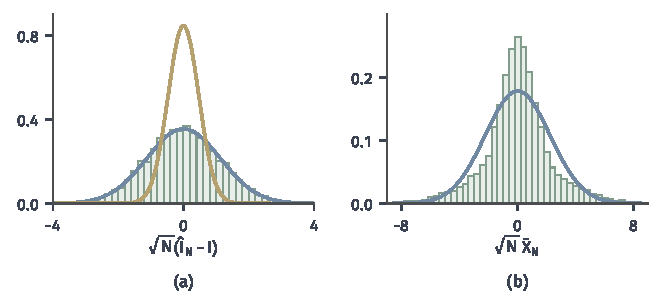
\includegraphics[width=112mm]{figures/07-probability/08-sampling-and-integration/matplotlib/mcerr-chain-clt/figure.pdf}
 \caption{链平均的极限分布。(a)两状态链$a=0.1$，$b=0.2$，从状态$0$出发，$N=2000$，$20000$条独立链（种子$3124$）的$\sqrt{N}(\hat{I}_N-1/3)$（绿色直方图），蓝线为$\mathcal{N}(0,34/27)$，黄线为误用单值方差的$\mathcal{N}(0,2/9)$；(b)可约链$(W,Y)$的$\sqrt{N}\hat{I}_N=WZ$的$20000$次抽样（绿色，种子$3125$），蓝线为$\mathcal{N}(0,5)$。}
 \label{fig:mcerr-chain-clt}
\end{BookInlineFigure}

\subsection{长期方差的估计}
\label{sec:mcerr-lrv-estimation}

即使中心极限定理成立，误差区间还需要$\sigma_{\mathrm{LR}}^{2}$的值。普通样本方差$S_N^{2}$估计的是$\gamma_0$，不是$\sigma_{\mathrm{LR}}^{2}$；用$S_N^{2}/N$作链平均的方差，在正相关时会把误差低估。下面两种估计都从同一条记录出发，分别从“分块”和“求和”两个方向逼近长期方差。

\paragraph{批均值}
由定理~\ref{thm:mcerr-long-run-limit}，长度为$b$的一段平稳记录，其平均的方差约为$\sigma_{\mathrm{LR}}^{2}/b$。若$b$远大于相关性的持续长度，相隔一段的两段平均几乎不相关。把记录切成$a$段，每段长$b$，$N=ab$，第$j$段的平均记为$\bar{Y}_j$。这$a$个段均值近似为方差$\sigma_{\mathrm{LR}}^{2}/b$的独立观测，于是它们的样本方差乘以$b$就估计了$\sigma_{\mathrm{LR}}^{2}$：
\begin{equation}
 \hat{\sigma}_{\mathrm{BM}}^{2}=\frac{b}{a-1}\sum_{j=1}^{a}\bigl(\bar{Y}_j-\hat{I}_N\bigr)^{2} .
 \label{eq:mcerr-batch-means}
\end{equation}
这种方法称为\term{批均值法}（batch means method）。$b=1$时每段只有一个值，式~\eqref{eq:mcerr-batch-means}退回普通样本方差$S_N^{2}$。

下面用一段短记录演示计算。两状态链（$a=0.1$，$b=0.2$）从不变分布出发运行$16$步（种子$3144$），$f$为状态$1$的示性函数，记录为
\[
 0,0,0,0,\ 0,0,1,0,\ 1,1,1,1,\ 1,0,0,0 .
\]
其中有六个$1$，$\hat{I}_{16}=6/16=0.375$。先算普通样本方差：六个值与平均相差$0.625$，十个值相差$-0.375$，
\[
 S_{16}^{2}=\frac{6\times0.625^{2}+10\times0.375^{2}}{15}=\frac{3.75}{15}=0.25 .
\]
再取段长$4$，分成四段，如图~\ref{fig:mcerr-batches}。段均值为
\[
 \bar{Y}_1=0,\quad \bar{Y}_2=0.25,\quad \bar{Y}_3=1,\quad \bar{Y}_4=0.25 .
\]
它们与$\hat{I}_{16}$的差的平方和为
\[
 0.375^{2}+0.125^{2}+0.625^{2}+0.125^{2}=0.5625 ,
\]
代入式~\eqref{eq:mcerr-batch-means}，
\[
 \hat{\sigma}_{\mathrm{BM}}^{2}=\frac{4}{3}\times0.5625=0.75 .
\]
两种估计给出的标准误差分别是
\[
 \sqrt{0.25/16}=0.125,\qquad \sqrt{0.75/16}=0.217 .
\]
真实的$\sigma_{\mathrm{LR}}^{2}=1.259$，平稳时的标准误差为$\sqrt{1.259/16}=0.281$。普通样本方差把它低估了一半以上；批均值的方向是对的，但只有四段，估计本身很粗糙。

\begin{BookInlineFigure}
 \centering
 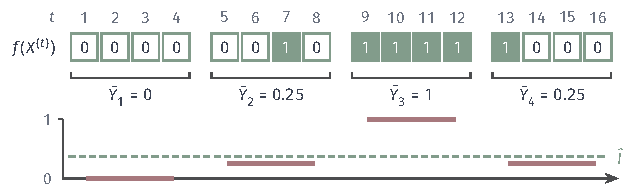
\includegraphics[width=107mm]{figures/07-probability/08-sampling-and-integration/tikz/mcerr-batches/figure.pdf}
 \caption{批均值的计算。上排为两状态链$16$步的函数值$f(X^{(t)})$（绿色方格为$1$），按长度$4$分成四段；下方红色横线为各段平均$\bar{Y}_j$，绿色虚线为总平均$\hat{I}=0.375$。段均值之间的离散程度反映了长期方差。}
 \label{fig:mcerr-batches}
\end{BookInlineFigure}

\paragraph{截断的自协方差和}
另一条路是直接按定义~\ref{def:mcerr-long-run}求和。由记录估计自协方差
\[
 \hat{\gamma}_k=\frac1N\sum_{t=1}^{N-k}\bigl(f(X^{(t)})-\hat{I}_N\bigr)\bigl(f(X^{(t+k)})-\hat{I}_N\bigr) ,
\]
再截断到$L$步：
\begin{equation}
 \hat{\sigma}_{L}^{2}=\hat{\gamma}_0+2\sum_{k=1}^{L}w_k\,\hat{\gamma}_k .
 \label{eq:mcerr-truncated-sum}
\end{equation}
权重$w_k=1$是直接截断；取$w_k=1-k/(L+1)$可以保证估计非负。不能对所有$k\leq N-1$求和：大$k$的$\hat{\gamma}_k$只由很少几对数据算出，噪声很大，全部加起来以后误差不随$N$缩小。

\paragraph{块长与截断的选择}
两种估计都面临同一个取舍。块长$b$或截断$L$太小，漏掉了尚未衰减的相关，估计偏低；太大，段数太少或加入太多噪声项，估计波动很大。图~\ref{fig:mcerr-lrv-estimates}在链~\eqref{eq:mcerr-ar1}（$\rho=0.9$）上用十条长度$2^{16}$的记录演示：$b=1$时批均值约为$\gamma_0=1$；$b=128$时十次的平均为$17.7$，仍偏低；$b=512$时平均为$18.7$，十次的标准差为$1.6$；$b=4096$时只剩$16$段，标准差增大到$7.9$。截断和的情形相同，$L$约为$60$时最稳定。

\begin{BookInlineFigure}
 \centering
 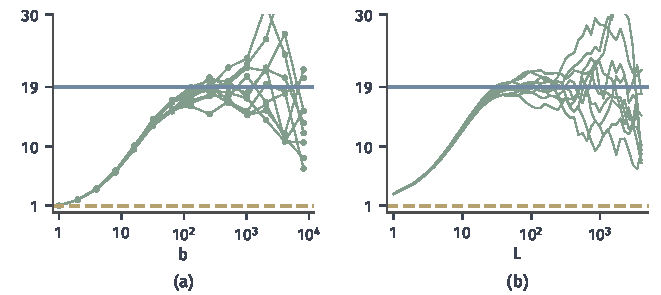
\includegraphics[width=112mm]{figures/07-probability/08-sampling-and-integration/matplotlib/mcerr-lrv-estimates/figure.pdf}
 \caption{长期方差的两种估计，链~\eqref{eq:mcerr-ar1}，$\rho=0.9$，$f(x)=x$，十条长度$N=2^{16}$的平稳记录（绿线，种子$3130$）。(a)批均值估计随块长$b$的变化；(b)直接截断的自协方差和随截断步数$L$的变化。蓝线为$\sigma_{\mathrm{LR}}^{2}=19$，黄色虚线为$\gamma_0=1$，横轴为对数刻度。}
 \label{fig:mcerr-lrv-estimates}
\end{BookInlineFigure}

要使估计一致，$b$与$a=N/b$都必须随$N$趋于无穷，例如$b$取$\sqrt{N}$的量级；截断和则要求$L\to\infty$且$L/N\to0$。此外还需要链以足够快的速度遍历，$f$满足比二阶更高的矩条件。证明需要把链的部分和与连续时间的随机路径作细致比较，超出本卷范围。

\paragraph{链平均的误差区间}
把三块拼起来：只有在链平均满足中心极限定理、$\sigma_{\mathrm{LR}}^{2}>0$且$\hat{\sigma}^{2}$是一致估计时，由Slutsky定理，
\[
 \frac{\sqrt{N}\,(\hat{I}_N-I)}{\hat{\sigma}}\xrightarrow{\mathrm{d}}\mathcal{N}(0,1) ,
\]
从而区间$\hat{I}_N\pm z\hat{\sigma}/\sqrt{N}$的覆盖概率趋于$1-\alpha$。这里的$\hat{\sigma}^{2}$是$\hat{\sigma}_{\mathrm{BM}}^{2}$或$\hat{\sigma}_{L}^{2}$，不能用$S_N^{2}$代替。三个条件中任何一个不成立，区间都没有保证：可约链没有正态极限，周期链可能$\sigma_{\mathrm{LR}}^{2}=0$，块长不当则方差估计不一致。

\subsection{运行诊断的边界}
\label{sec:mcerr-diagnostics}

上面的条件涉及链的遍历性质，通常无法从记录中验证。实践中用一些运行诊断来发现问题，它们各有用处，也各有盲区。

\paragraph{一个双峰目标}
取$\pi$为$\mathcal{N}(-5,1)$与$\mathcal{N}(5,1)$的等权混合，$f(x)=x$，$I=0$。用第~\ref{chap:sample-generation}章的随机游走Metropolis算法：从当前状态$x$提出候选$y=x+\eta$，$\eta\sim\mathcal{N}(0,1)$，以概率$\min\{1,\tilde{p}(y)/\tilde{p}(x)\}$接受，否则留在$x$，其中$\tilde{p}$是$\pi$的密度。这条链以$\pi$为不变分布，并且候选可以到达任何位置，理论上能在两个峰之间往返。问题在于两峰之间密度很低：$x=0$处的密度只有峰值的$2\mathrm{e}^{-12.5}\approx7\times10^{-6}$倍，每一步只能移动一个单位左右，穿越低谷需要连续多次接受向下的移动，这几乎不会发生。

图~\ref{fig:mcerr-bimodal-traces}(a)从$-7,-3,3,7$出发运行四条链，每条$5000$步（种子$3131$），接受率约为$0.70$。四条链没有一次穿过$0$：两条留在左峰，平均为$-5.00$与$-5.01$；两条留在右峰，平均为$5.05$与$4.95$。链间的分歧明白地暴露了问题。把四条链合在一起，平均为$-0.004$，碰巧接近$0$，但这只是因为初值恰好两边各两个；若三条从左边出发，合并平均就在$-2.5$附近。两峰各占多少质量，这些记录完全没有测量到。

图(b)把四条链都放在左侧，从$-7,-6,-4,-3$出发（种子$3132$）。四条链的平均分别为$-4.98,-4.98,-5.03,-4.94$，彼此一致；轨迹看起来平稳，运行平均早已停住，每条链的估计有效样本量也不小。所有诊断都通过了，答案却是$-4.98$而不是$0$。

\begin{BookInlineFigure}
 \centering
 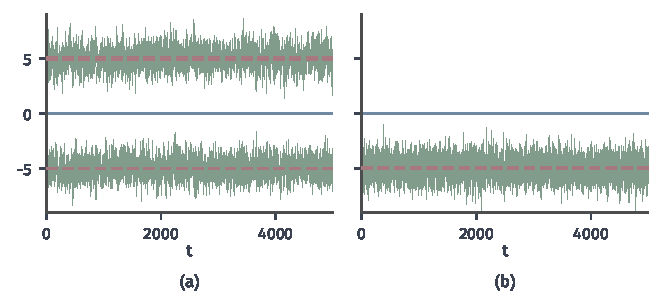
\includegraphics[width=112mm]{figures/07-probability/08-sampling-and-integration/matplotlib/mcerr-bimodal-traces/figure.pdf}
 \caption{双峰目标$\frac12\mathcal{N}(-5,1)+\frac12\mathcal{N}(5,1)$上的随机游走Metropolis链，每条$5000$步。绿线为轨迹，红色虚线为每条链的平均，蓝线为$I=0$。(a)从$-7,-3,3,7$出发（种子$3131$）；(b)从$-7,-6,-4,-3$出发（种子$3132$）。}
 \label{fig:mcerr-bimodal-traces}
\end{BookInlineFigure}

\paragraph{各种诊断能看到什么}
表~\ref{tab:mcerr-diagnostics}总结了常用的几种诊断。比较多次运行时，常同时看链间平均的差异与链内的波动：若链间差异远大于链内波动所能解释的范围，说明各链还没有忘掉初值或停在不同区域。\term{轨迹图}（trace plot）即状态随步数的曲线，\term{运行均值}（running mean）即前$t$步平均随$t$的曲线。

\begin{BookInlineTable}
 \centering
 \caption{运行诊断的作用与盲区}
 \label{tab:mcerr-diagnostics}
 \begin{tabular}{p{25mm}p{36mm}p{36mm}}
  \toprule
  诊断 & 能发现 & 不能发现 \\
  \midrule
  不同初值的多次运行 & 初值影响，停在不同区域 & 所有初值都未到达的区域 \\
  轨迹图 & 趋势，缓慢移动，停滞 & 从未访问的区域 \\
  运行均值 & 尚未稳定的漂移 & 稳定在错误值上 \\
  估计的有效样本量 & 强相关，方差估计不稳 & 只在局部区域混合良好 \\
  \bottomrule
 \end{tabular}
\end{BookInlineTable}

这些诊断共同的盲区是：有限的记录只能告诉我们链去过哪里，不能告诉我们还有哪里没去。双峰例子里，记录中没有任何信息提示右边还有一半质量；第~\ref{sec:mcerr-asymptotic-interval}小节的稀有大贡献是同一现象在独立样本中的版本。所以诊断的结论只能是否定性的：诊断失败说明有问题，诊断通过不说明没有问题。误差区间所需的遍历性与矩条件，需要从目标与转移的结构分析得到，例如知道目标的峰在哪里，或者证明转移满足几何遍历；运行诊断不能替代这些理论条件。
